%% Change "letterpaper" in the following line to "a4paper" if you must.

\documentclass[10pt,letterpaper]{article}

\usepackage{cogsci}
\usepackage{pslatex}
\usepackage{apacite}
\usepackage{subcaption}
\usepackage{graphicx}
\usepackage{amsmath}
\usepackage{relsize}
\usepackage{natbib}
\usepackage{float}

\floatstyle{boxed}
\restylefloat{figure}


\title{Analogies Emerge from Learning Dyamics in Neural Networks}
 
\author{{\large \bf Andrew Lampinen (lampinen@stanford.edu)} \\
  Department of Psychology, Jordan Hall, 450 Serra Mall, Stanford CA 94305 
  \AND {\large \bf Shaw Hsu (cshawhsu@stanford.edu)} \\
  Department of Biophysics, James H. Clark Center, 318 Campus Dr., Stanford CA 94305
  \AND {\large \bf James L. McClelland (mcclelland@stanford.edu)} \\
  Department of Psychology, Jordan Hall, 450 Serra Mall, Stanford CA 94305} 


\begin{document}

\maketitle


\begin{abstract}
Neural networks have been shown to extract analogous structure from tasks which do not share inputs or outputs. This may explain the value of multi-task training, and also may underlie the power of human analogical reasoning -- rather than an advanced cognitive ability requiring symbolic computation, analogy may be simply a natural feature of learning in neural networks. We generalize linear analysis techniques that have proven helpful in analyzing non-linear networks to explore two tasks, show that analogous structure is commonly extracted, and address some potential implications. 

\textbf{Keywords:} 
neural networks; structure learning; representation; analogy; transfer; 
\end{abstract}


\section{Introduction}
Neural networks are capable of extracting analogous structure from knowledge domains that are completely non-overlapping in their inputs and outputs \citep{Hinton1986,Rogers2008}. This sets them apart from simple forms of statistical pattern recognition \citep{Rogers2008} such as linear data analysis techniques like PCA. However, there have been important theoretical developments in linear neural networks recently which have been shown to have applications to understanding learning in non-linear neural networks \citep{Saxe2013}. How can we employ the full power of non-linear neural networks while still gaining insight from linear analysis techniques? Do neural networks commonly extract shared structure when solving tasks?\par 
\subsection{Why Should We Care?}
Why might analogy extraction be important? Analogy is often considered an essential part of human cognition \cite[e.g.]{Gentner2003}. When neural networks form representations which reflect analogous structures, this can support analogy \citep{Pennington2014,Kollias2013}. This may explain how analogies can emerge intuitively in the human mind without the computationally expensive search often used in analogical reasoning systems \cite[e.g.]{Falkenhainer1989}. \par
In addition, multi-task learning has proven beneficial for producing efficient learning and effective generalization in neural networks on a variety of tasks, \cite[e.g.]{Dong2015,Rusu2015}. Even a small amount of learning on distinct but related tasks has been shown to improve performance. For example, training a natural language translation system on image captioning and autoencoding improves translation performance \citep{Luong2016}. Learning on numerous language translation pairs can even give generalization without further training to unseen language pairs \citep{Johnson2016a}. Because human experience is filled with distinct tasks that share common elements (language, various perceptual modalities, etc.) the way that structure is learned across tasks may be essential to understanding human intelligence and building better artificial intelligence systems.\par
However, we have little understanding of how, why, or when neural networks are able to extract ``hidden'' analogous structure like this. Here, we describe a preliminary investigation into this question, and in the process describe a new approach to analyzing neural network representations that may yield more general insights. 
\section{A Simple Task}
In the original work of \citet{Hinton1986}, a neural network was taught to answer queries about the structure of two perfectly analogous family trees (one English and one Italian, see fig. \ref{hinton_family_tree_figure}), and was shown to generate representations that extract the analogy, in the sense that analogous people from different families are represented similarly. Here, we pare this task down to its barest essentials: two perfectly analogous domains with separate inputs and ouputs. For our task, the inputs can be thought of as the set of letters \(\{R,L,\rho,\lambda\}\), and the outputs as \(\{P,D,S,\pi,\delta,\sigma\}\). The task can be seen as mapping an input letter onto the letters that it can follow (e.g. ``R'' can follow ``D'' as in ``draw,'' but cannot follow ``S''), where there is an analogy between the Latin and Greek letters. See below for the input-output (I/O) mapping: 
\[
\begin{array}{c|cccccc} 
& P & D & S & \pi & \delta & \sigma \\
\hline
R & 1 & 1 & 0 & 0 & 0 & 0 \\
L & 1 & 0 & 1 & 0 & 0 & 0 \\
\rho & 0 & 0 & 0 & 1 & 1 & 0\\
\lambda & 0 & 0 & 0 & 1 & 0 & 1\\
\end{array} 
\]
We trained a neural network with a single hidden layer (4 units) to solve this task. See fig. \ref{network_diagram} for a diagram of the network. No biases were used, weights were initialized randomly between 0 and 0.1, all training was done by Stochastic Gradient Descent (i.e. in each epoch the data are presented one at a time in a random order, and the weights are updated after each data point) with \(\eta = 0.01\) for 500 epochs. We include only a single non-linearity (a rectifier) at the output layer. When and how does this simple network extract the analogous structure across the domains? \par
\begin{figure*}
\centering
\begin{subfigure}{0.22\textwidth}
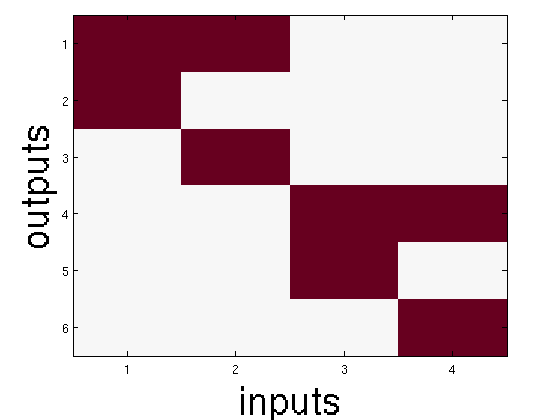
\includegraphics[width=\textwidth]{figures/nonlinear_IO.png}
\caption{$\Sigma_{IO,nl}$}
\end{subfigure}
\huge{$=$}
\begin{subfigure}{0.22\textwidth}
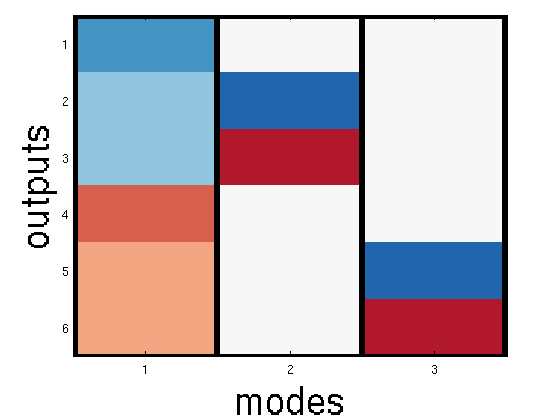
\includegraphics[width=\textwidth]{figures/U_nl.png}
\caption{$U_{nl}$}
\end{subfigure}
\LARGE{$\times$}
\begin{subfigure}{0.22\textwidth}
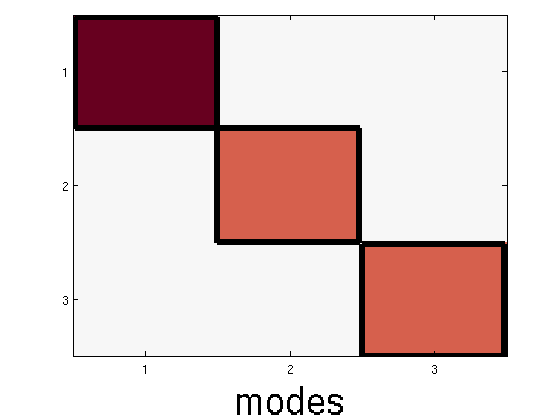
\includegraphics[width=\textwidth]{figures/S_nl.png}
\caption{$S_{nl}$}
\end{subfigure}
\LARGE{$\times$}
\begin{subfigure}{0.22\textwidth}
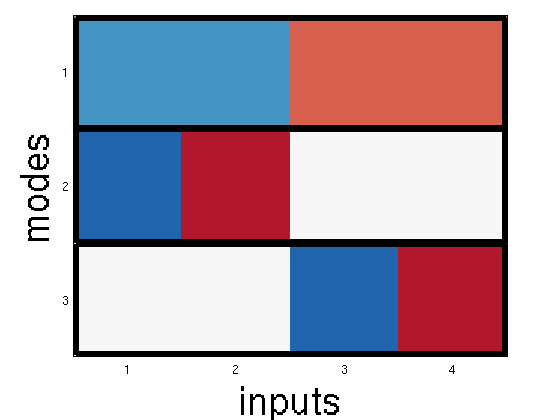
\includegraphics[width=\textwidth]{figures/V_nl.png}
\caption{$V_{nl}$}
\end{subfigure}
\caption{SVD of I/O correlation matrix (colors are scaled to show qualitative features, red = +, white = 0, blue = -)}
\label{regular_SVD_figure}
\end{figure*}
\subsection{Linear Analysis?}
As mentioned above, there have been recent developments in the theory of linear neural networks which show that the process of learning is entirely driven by the Singular Value Decomposition (SVD) of the input-output correlation matrix \citep{Saxe2013}. These results have been shown to have implications for the learning of non-linear networks as well, so linear neural networks can be a more tractable place to analyzee learning dynamics. In addition, using the I/O SVD allows the discovery of representational components which are distributed across units, so it is more general than simply examining what aspects of the task individual hidden units represent, or examining the weight matrices directly. Thus one might hope to answer our questions in a linear framework. \par
However, linear networks cannot represent analogous structure from non-overlapping inputs and outputs at convergence. With non-overlapping inputs and outputs, the I/O correlation matrix is block diagonal, and the SVD modes will thus occur within blocks (see Fig. \ref{regular_SVD_figure} for a demonstration of this on our task). Thus, since the final representational components that a linear network learns are precisely the components of the SVD \citep{Saxe2013}, there will not be any sharing of structure across domains.\par 
Furthermore, the optimal rank $k$ approximation to a matrix is to take the top $k$ components from the SVD \citep{Mirsky1960}. If a linear network's hidden layers are restricted to rank lower than that of the I/O correlation matrix, detail within the domains will be lost. Thus a linear neural network cannot solve the task perfectly if any of its hidden layers has a number of units smaller than the rank of the I/O correlation matrix. By contrast, a non-linear network can exploit the analogy between the domains to find more parsimonious solutions. Is there a way to leverage linear insights in the non-linear case?  
\begin{figure*}
\centering
\begin{subfigure}{0.22\textwidth}
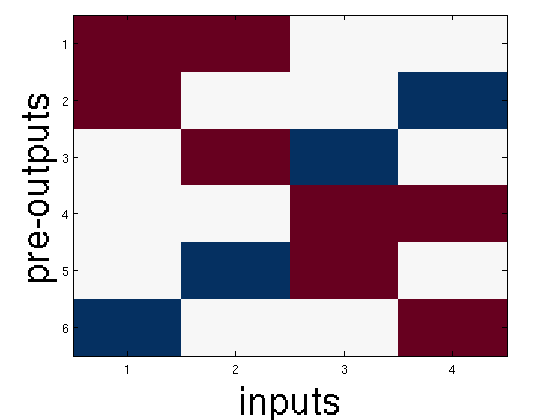
\includegraphics[width=\textwidth]{figures/linearized_IO.png}
\caption{$\Sigma_{IO,lz}$}
\end{subfigure}
\huge{$=$}
\begin{subfigure}{0.22\textwidth}
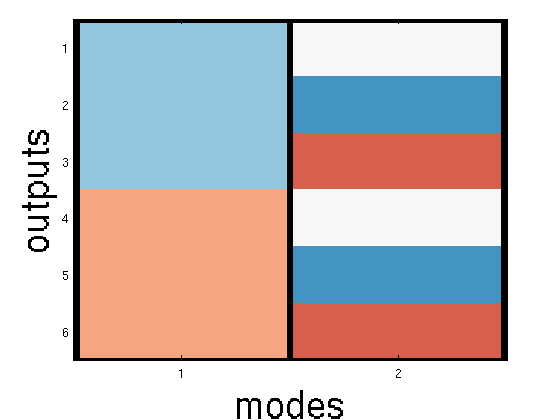
\includegraphics[width=\textwidth]{figures/U_lz.png}
\caption{$U_{lz}$}
\end{subfigure}
\LARGE{$\times$}
\begin{subfigure}{0.22\textwidth}
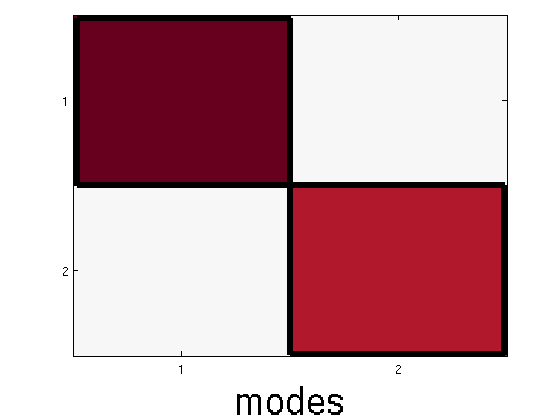
\includegraphics[width=\textwidth]{figures/S_lz.png}
\caption{$S_{lz}$}
\end{subfigure}
\LARGE{$\times$}
\begin{subfigure}{0.22\textwidth}
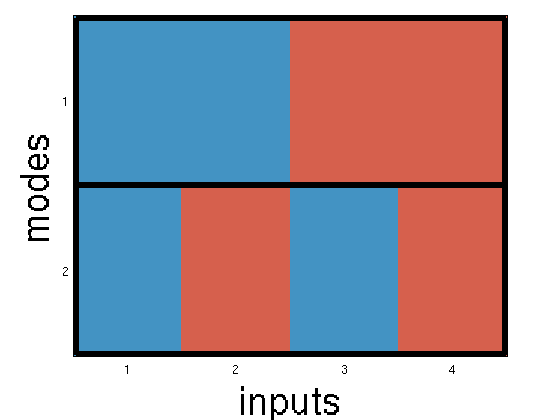
\includegraphics[width=\textwidth]{figures/V_lz.png}
\caption{$V_{lz}$}
\end{subfigure}
\caption{SVD of linearized I/O correlation matrix (colors are scaled to show qualitative features, red = +, white = 0, blue = -)}
\label{linearized_SVD_figure}
\end{figure*}
\subsection{A Linearized Approach}
\begin{figure}[p]
\centering
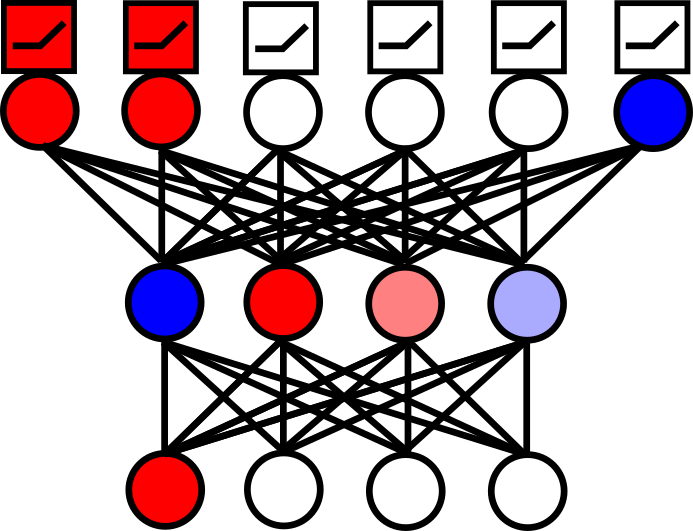
\includegraphics[width=0.22\textwidth]{figures/network_diagram.png}
\caption{Simple task network, showing a sample propagation of an input through the network with the single non-linearity at the output. (Circles represent inputs or fully connected units, squares represent non-linearities.) }
\label{network_diagram}
\end{figure}
As we shall see, while a linear network cannot extract the analogous structure from the task, inserting a single non-linearity after the output layer can allow it to do so. In the case that the non-linearity is a sigmoid, this essentially reduces the problem to logistic regression; here we will use rectified linear units in our analysis because their structure makes the output patterns more intuitively interpretable. Once this almost-linear network has solved the problem, consider its outputs immediately prior to the non-linearity. These are produced by the linear part of the network, and together with the non-linearity suffice to produce the desired outputs. We can use these to turn the problem into a linearly analyzable one -- simply treat these pre-nonlinearity outputs as outputs of a linear network. Then the problem becomes susceptible to the types of linear analyses discussed above. We will refer to this as the ``linearized'' version of the network. \par 
In the simple task described above, the solution that the nonlinear network discovers the majority of the time (about 75\%) is to output the same pattern on both sets of output units, but offset the ``incorrect'' domain sufficiently negative so that the output after the rectifier is zero, thus transforming the I/O mapping into a linearized I/O mapping as follows: \par
\vspace{-1em}
{ \relsize{-1}
\[
\left[ \begin{matrix} 
1 & 1 & 0 & 0 & 0 & 0 \\
1 & 0 & 1 & 0 & 0 & 0 \\
 0 & 0 & 0 & 1 & 1 & 0\\
 0 & 0 & 0 & 1 & 0 & 1\\
\end{matrix}  \right] 
\mathlarger{\mathlarger{\Rightarrow}}
\left[ \begin{matrix} 
1 & 1 & 0 & 0 & 0 & -1 \\
1 & 0 & 1 & 0 & -1 & 0 \\
 0 & 0 & -1 & 1 & 1 & 0\\
 0 & -1 & 0 & 1 & 0 & 1\\
\end{matrix}  \right] 
\] }
(Note that the network can actually map the first element of one domain onto either element of the other, since they are perfectly symmetrical. This solution occurs as well, but we discuss the one shown here for clarity, the other solution just shuffles some rows and columns.) We can use this linearized I/O mapping to perform a linear analysis. When the SVD of this linearized I/O correlation matrix is evaluated, a rank 2 solution emerges. The components of the linearized SVD are (qualitatively): \begin{enumerate}
\itemsep-0.25em
\item The separation of the domains
\item The analogous structure within the domains
\end{enumerate}
(see fig. \ref{linearized_SVD_figure}). The first component is similar to the first component of the regular SVD, in that it reflects the separation of the domains, but the second component collapses the two components of the linear SVD. In other words, the analogy has been learned. Thus a network with a single non-linearity is able to represent the analogy by allowing the outputs in both domains to vary, and simply suppressing the output from the ``wrong'' domain for the current task.\par
Furthermore, because this solution is rank 2, a non-linear network with two hidden units should be able to solve the task, whereas a linear network will require at least 3. We have verified these results empirically for this task -- a non-linear network is always able to solve the task with only 2 hidden units, while a linear network did not solve it with fewer than 3 hidden units. Thus the ability of a non-linear neural network to extract common structure from multiple tasks can allow it to find lower-rank (i.e. more parsimonious) solutions. 
\subsection{Evolution of the I/O Mappings}
%\begin{figure}
%\centering
%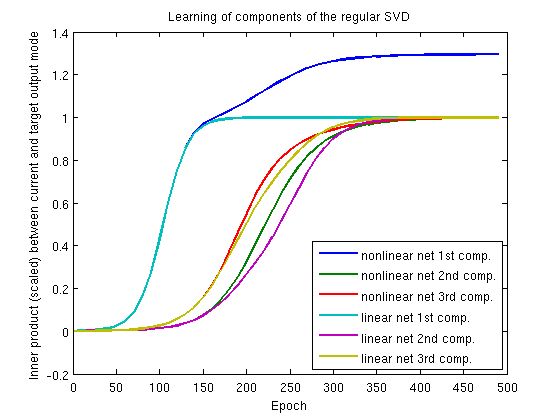
\includegraphics[width=0.5\textwidth]{figures/regular_SVD_component_learning.png}
%\caption{I/O SVD component learning (dot product between output mode of an SVD component and the response of the network to the corresponding input mode, scaled by the corresponding singular value)}
%\label{regular_SVD_component_learning}
%\end{figure}
%
%\begin{figure}
%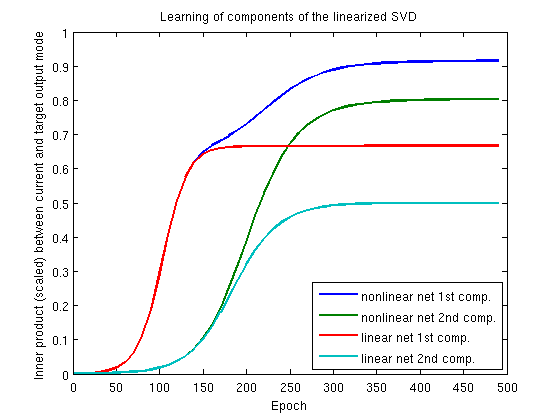
\includegraphics[width=0.5\textwidth]{figures/linearized_SVD_component_learning.png}
%\caption{Linearized I/O SVD component learning (dot product between output mode of an SVD component and the response of the network to the corresponding input mode, scaled by the corresponding singular value)}
%\label{linearized_SVD_component_learning}
%\end{figure}
\begin{figure}
\centering
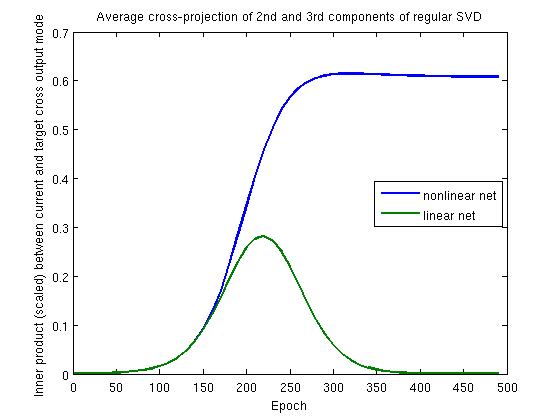
\includegraphics[width=0.5\textwidth]{figures/SVD_cross_projection_learning.png}
\caption{I/O SVD component cross-projection (dot product between output mode of an SVD component and the response of the network to the \textbf{other domain's} input mode)}
\label{SVD_cross_projection_learning}
\end{figure}
\begin{figure}
\centering
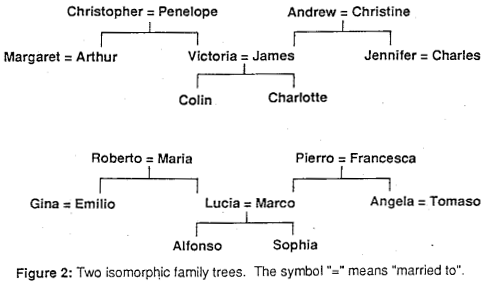
\includegraphics[width=0.35\textwidth]{figures/hinton_family_tree_figure.png}
\caption{Family trees from \citet{Hinton1986}, (permission pending).}
\label{hinton_family_tree_figure}
\end{figure}
\begin{figure}
\centering
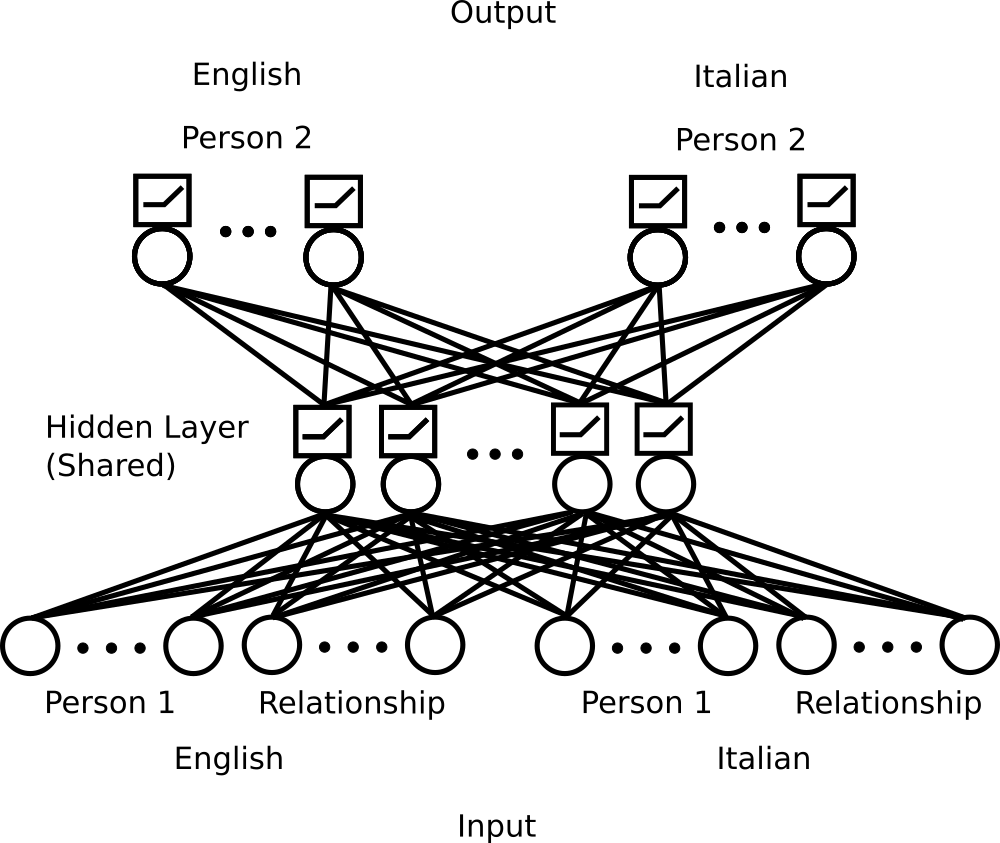
\includegraphics[width=0.43\textwidth]{figures/family_tree_network_diagram.png}
\caption{Family tree task network (Circles represent inputs or fully connected units, squares represent non-linearities. Ellipses denote units omitted from the diagram -- the hidden layer and all input and output groups had 12 units apiece.)}
\label{family_tree_network_diagram}
\end{figure}
When a non-linear network has only two hidden units, it must extract the analogy to be able to solve the task, but with more hidden units there are a variety of solutions that could potentially emerge (such as just learning the mapping of each input to its output pattern independently). However on a set of 100 runs we conducted, a non-linear network with 4 hidden units extracted shared structure on about 75\% of them (as measured by more than 20\% score on the cross-projection metric described below). What drives this fairly consistent emergence of representations that reflect the analogous structure? In this section we consider the evolution of the representations and outputs over the course of learning on this simple task. \par 
The output structure of the network goes through a fairly consistent progression, which we will describe qualitatively in terms of the general structure of the input-output mapping at various epochs (the exact values depend on the initialization, so the matrices here are approximations to within about \(\pm 0.1\)). The outputs begin as small positive numbers, approximately 0 (because the weights are initialized uniformly between 0 and 0.1). Next, the network captures the base rate activations of each output unit, around epoch 75. (Note that this step is already accounted for in the SVD, because the output variables are centered before taking the SVD). \par
{ \relsize{-1}
\[ 
\text{base rates} = \left[ \begin{matrix} 
0.5 & 0.25 & 0.25 & 0.5 & 0.25 & 0.25 \\
\vdots & \vdots &\vdots &\vdots &\vdots &\vdots \\
 0.5 & 0.25 & 0.25 & 0.5 & 0.25 & 0.25\\
\end{matrix}  \right] 
\] 
}
Then the network captures the existence of the two domains but not the structure within them (around epoch 140). This corresponds to the first component of either SVD. Up to this point, a linear network follows a similar learning trajectory. \par
\vspace{-1em}
{ \relsize{-1}
\[
\text{base rates by domain} = \left[ \begin{matrix} 
1 & 0.5 & 0.5 & 0 & 0 & 0 \\
1 & 0.5 & 0.5 & 0 & 0 & 0 \\
0 & 0 & 0 & 1 & 0.5 & 0.5  \\
0 & 0 & 0 & 1 & 0.5 & 0.5  \\
\end{matrix}  \right] 
\] 
}
Finally it learns the internal structure of the domains (they are not learned at exactly the same time, which is learned first depends on the initilization). Around epoch 400 it has solved the task completely, with some sort of offset structure in the non-linear case, or without in the linear case:\par
\vspace{-0.5em}
{ \relsize{-1}
\[
\text{solution with offsets} = \left[ \begin{matrix} 
1 & 1 & 0 & 0 & 0 & -1 \\
1 & 0 & 1 & 0 & -1 & 0 \\
 0 & 0 & -1 & 1 & 1 & 0\\
 0 & -1 & 0 & 1 & 0 & 1\\
\end{matrix}  \right] 
\]
}
For most of the learning process, the networks are extracting similar structure, so one might expect that even the linear network would show some representation of the analogy at intermediate stages of learning. Indeed, once the base rates by domain are learned, both the linear and non-linear networks begin to extract the analogy between the domains. See fig. \ref{SVD_cross_projection_learning} for a plot of how much each domain's input mode projects to the \textbf{other domain's} output mode, i.e. ``cross-talk'' between the domains. This measures the extent to which the network is extracting shared structure. However, while both networks develop some representation of the analogy initially, this activity extinguishes rapidly within the linear network, while it stabilizes at a positive value in the non-linear network. \par
Why do both networks show some representation of the analogy initially? We will analyze this in the linear case. At the stage when the base rates by domain have been learned, adding a little bit of shared structure actually reduces mean-squared error (MSE). If the network moves from the base rates by domain pattern to the pattern shown below, the small increase in MSE from the \(\pm 0.1\) values is more than offset by the decrease from splitting the 0.5 values into 0.4 and 0.6. \par 
{ \relsize{-1}
\[
\left[ \begin{matrix} 
1 & 0.6 & 0.4 & 0 & 0.1 & -0.1 \\
1 & 0.4 & 0.6 & 0 & -0.1 & 0.1 \\
0 & 0.1 & -0.1 & 1 & 0.6 & 0.4  \\
0 & -0.1 & 0.1 & 1 & 0.4 & 0.6  \\
\end{matrix}  \right] 
\] 
}
Indeed, suppose there is any hidden unit which responds differentially within the domains (as they all will to some extent because of the random initialization). The updates of the output weights for this unit will naturally point in the direction of analogy extraction once the base rates by domain have been learned. See below for the output error, hidden unit activity, and corresponding weight updates in the case that the hidden unit responds positively to the first element of each domain, and negatively to the other.\footnote{Of course, in the general case representations will be distributed across the hidden units, and so there will not be a unit which responds slightly to the analogy and nothing else, but this is simply a rotation of the representation space, and because of the linearity of derivatives the same general pattern will emerge.} (Note that the output weight updates for a hidden unit are proportional to the product of the output error and the hidden unit's activation.) \par
\vspace{-1em}
{ \relsize{-1}
\[
\begin{array}{cccccc||c||cccccc} 
\multicolumn{6}{c||}{\text{output error}}  & \text{unit}  & \multicolumn{6}{c}{\text{unit output weight updates}} \\
\hline
 0 & + & - & 0 & 0 & 0  &   +    &  0 & + & - & 0 & 0 & 0   \\
0 & - & + & 0 & 0 & 0  &   -  & 0 & + & - & 0 & 0 & 0   \\
 0 & 0 & 0 & 0 & + & - &   +   &  0 & 0 & 0 & 0 & + & - \\
 0 & 0 & 0 & 0 & - & +  &  - &  0 & 0 & 0 & 0 & + & - \\
\hline
\multicolumn{7}{r}{\text{net output weight update:}} &   0 & + & - & 0 & + & - \\
\end{array} 
\]
}
Summing these updates across the four patterns naturally captures the analogy between the domains. The network will exploit this analogy to reduce error, even if it must eventually discard it in the linear case.\footnote{ Why does this structure die out in the linear network but persist in the non-linear one? In the linear network, as mentioned above, the optimal solution the network must reach is precisely the linear SVD. Since the components of the linear SVD do not have shared structure, the linear network cannot represent analogous structure at convergence. By contrast, the non-linear network can simply offset the other domain's outputs further below zero, and thus make use of the analogy rather than being harmed by it.} \par 
\section{Reanalyzing Hinton's Family Tree Example}
\begin{figure}
\centering
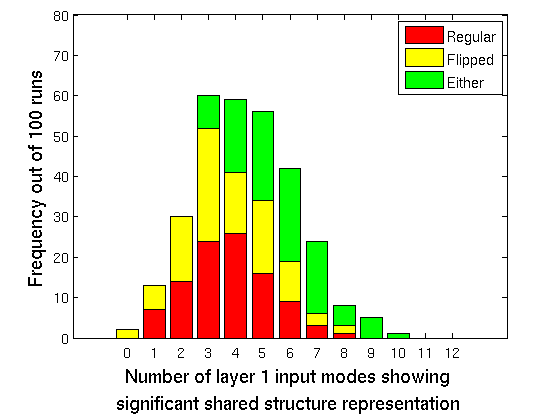
\includegraphics[width=0.5\textwidth]{figures/ft_input_mode_significance_hist.png}
\caption{How many of the input modes from the layer 1 SVD showed significantly more projection than would be expected onto the direct analogy between the families, the flipped analogy, or either of them (without double counting)}
\label{ft_input_mode_sig_hist}
\end{figure}
Next, we briefly turn our attention to the example of \citet{Hinton1986} which inspired this work. Hinton's task involves learning the structure of two isomorphic family trees, one English and one Italian (see fig. \ref{hinton_family_tree_figure}). This structure is taught implicitly by presenting a person (e.g. ``Jennifer'') and a relationship (e.g. ``Father''), and training the network to produce the correct target person (``Andrew'' in this case). There are 52 such relationships per family, for 104 total. Hinton used different inputs for each families members, but used the same relationship inputs for both families. To highlight the extraction of analogous structure we separated these into distinct inputs (these could be thought of as corresponding to the English and Italian words for different relations, e.g. ``uncle'' vs. ``zio'' ). We also reduced his network down from 3 hidden layers to a single hidden layer with 12 units. Unlike the simple problem above, the family tree problem is not linearly separable, so we included a non-linearity at the hidden layer as well as the output (see fig. \ref{family_tree_network_diagram}). We trained this network by SGD with \(\eta = 0.005\) for 1000 epochs. \par 
In a task which requires multiple non-linearities, we cannot perform as simple an analysis as in the earlier task. However, by definition each layer of the network has only a single non-linearity, and so we can perform an analysis like the above on each layer. In this way we can understand something about the computations that the network is performing and the structure it is extracting. However, the interpretation will not be as simple as in the single non-linearity case. \par
This difficulty is compounded by the complexity of the structure being learned in each family. In the simple problem above it was possible to ``eyeball'' the structure extraction, but here the structure is too rich. There are a variety of possible ways the families can be mapped onto one another (e.g. flipping the tree left to right and swapping all genders), and it's possible that the networks are extracting overlapping structure from several of these analogies. In this setting, how can we examine whether the network is learning the analogy? \par
%\begin{figure}[H]
%\centering
%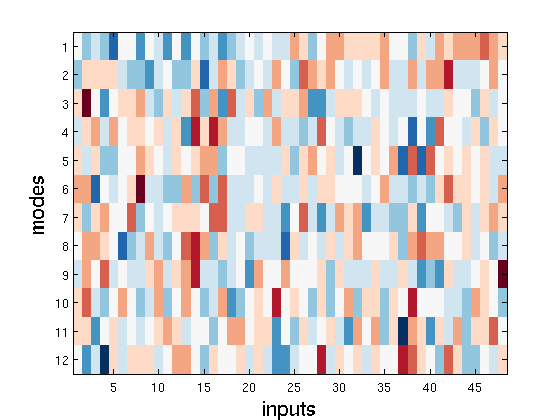
\includegraphics[width=0.5\textwidth]{figures/ft_input_mode_example.png}
%\caption{Example layer 1 SVD input modes from the family tree task}
%\label{ft_input_mode_example}
%\end{figure}
As a first test of this, we looked for representation of the analogy in the input modes of the first layer SVD. To do this, we computed the dot product of each mode's weights for one family with that mode's weights for the other family, and then tested how significant this similarity was by comparing it to the null distribution generated nonparametrically by randomly permuting the columns of the input mode matrix 1000 times and computing the same dot product for each one. We denoted a mode as showing significant extraction of the analogy if it showed a stronger similarity between the weights for the two families' inputs than 95\% of its permutations did. \par
We repeated this process across 100 network initilizations and found a great deal of analogous structure was being extracted. The runs had a median of 4 modes showing significant analogous structure extraction, and all the runs had at least one mode that showed it (for comparison, if 5\% of the modes showed significant results by chance, we would still expect 54\% of the runs to yield no significant results, and the median number of shared structure components would thus be zero). To account for the symmetry of the tree under flipping, we repeated the same analysis after permuting the second family's input columns to flip the tree. Since the network has no way to distinguish the ``regular'' mapping from this ``flipped'' mapping during learning, we would expect to see a similar frequency of modes which reflect the ``flipped'' analogy, and indeed the distribution is similar. Furthermore, the runs had a median of 6 modes showing significant extraction of the analogy to either the regular or flipped mapping, in 95\% of the runs the network had extracted 3 or more significant components from at least one of the mappings, and in all of the runs it had extracted 3 or more components that significantly represent one analogy or the other (if we assume 5\% false positives again, we would expect results this extreme in only 0.01\%, 4\% and 3\% of the runs, respectively). See fig. \ref{ft_input_mode_sig_hist}. \par
We performed a similar analysis for the output modes of layer 2, and again found a great deal of analogous structure extraction, though less than in the input modes of the first layer. The median number of modes that showed significant representation of analogous structure was 4, and in 64\% of the runs the network had extracted 3 or more significant components for at least one of the analogies. It is somewhat unsurprising that the output mappings would show less representation of structural analogies than the input mappings, since to solve the task the network must offset any shared structure in the output modes to prevent it appearing in the output. Still, the frequency with which the common structure is significantly represented, even in the output modes, suggests this is a central feature of how neural networks solve tasks. \par  
Although we have focused on broad analogies between the families here, analyzing the SVDs can give much more detailed information. The analogies can be analyzed in detail; in some cases modes reflect an analogy only in the ``person'' inputs, or only in the ``relationship'' inputs. Within a family, analyzing the SVD modes can outline the structure the network is extracting, e.g. modes often appear which represent the gender of the target of a relationship like ``mother''. We have omitted analyses like these for the sake of brevity. \par 
\section{Disussion}
We have outlined a new technique for analyzing neural network representations and their learning dynamics: analyzing the SVD of the ``linearized'' mapping at each layer (i.e. the mapping from the inputs to the pre-nonlinearity activity). This allows us to bring the power of linear analyses to bear on the rich phenomena that occur only in non-linear networks.\par
Using this technique, we have explored how a simple neural network can extract the analogy between tasks with non-overlapping inputs and outputs. We showed that a single non-linearity at the output layer of a neural network can allow the network to represent this common structure on a simple task, and that this structure emerges naturally (even in a linear network) from gradient descent once the base rates of the various domains have been learned. A linear network must discard this analogy to reach its optimal solution, but a non-linear network is able to retain it by simply offsetting the outputs to a sufficiently negative value, and does so the majority of the time in our results. Here we used rectifiers, but the same solution is achievable with sigmoid, tanh, etc. \par 
We then broadened our approach to explore the family tree task originally proposed in \citet{Hinton1986}. Because this task is not linearly separable, we created a general network with two nonlinear layers, and applied our analysis to each layer. We found evidence of a great deal of extraction of two possible analogies between the families in the network (either the intended isomorphism between the family trees, or one in which one family tree was flipped left-to-right and gender-reversed), and that networks seemed generally to be discovering elements of both analogies. Indeed, representation of the analogies seemed even more common than on the simpler task. On the simple task 25\% of the networks showed no evidence of common structure extraction, but on the family tree task every network extracted at least three input modes that projected significantly onto one of the analogies. \par 
These results suggest that rather than an advanced cognitive ability requiring symbolic computations, analogy may be simply a natural feature of gradient based learning in nonlinear neural networks. Furthermore, learning of analogous structure between tasks may facilitate more rapid learning and better performance on these tasks, as with the multi-task machine learning examples cited above. The power and generality of human cognition may result from extracting common structure from the diverse but deeply related tasks we engage in throughout our lives. 
\subsection{Future Directions}
\begin{enumerate}
\itemsep0em
%%\item When and why is analogous structure not extracted -- what features of the initilization cause this, and how does it interact with task complexity?
\item In our analysis of the family tree task we analyzed the input modes of the first layer and the output modes of the second layer. An important future direction will be exploring the modes which map into and out of the hidden layer, and what they imply about the representations at the hidden layer. This would also allow us to apply this analysis to deep networks. This is important, since recent developments have highlighted the importance of depth, and deep models are being used to understand the representations that emerge in the brain \citep[e.g.]{Yamins2016a}. We believe that these techniques will be applicable to deeper models without too much additional difficulty. 
\item We motivated this paper by discussing the importance of analogy in human reasoning. Some interesting questions:
\begin{itemize}
\itemsep0em
\item How do learning trajectories change with explicit cueing of the analogy (e.g. presenting analogous exemplars together, or using shared inputs for part of the domain, as \citet{Hinton1986} did in the family tree model), or when one domain is learned before another?
\item What happens when structures do not perfectly match, as is the case in most real world analogies?
\item The fact that neural networks learning by gradient descent consistently and automatically extract analogies hidden within their inputs suggests that in effect this process may serve as automatic amortized inference about potential analogical structures in the world. Can this explain the power of human analogical reasoning?  
\end{itemize}
\end{enumerate}
\section{Acknowledgments}
This material is based upon work supported by the NSF GRF under Grant No. DGE-114747.
\bibliographystyle{apacite}

\setlength{\bibleftmargin}{.125in}
\setlength{\bibindent}{-\bibleftmargin}

\bibliography{shared_reps}


\end{document}
